\documentclass[12pt]{article}
\usepackage{reportNTU}
\usepackage{siunitx}

\definecolor{ntuBlue}{RGB}{0,70,140}
\definecolor{softBlue}{RGB}{232,241,250}
\definecolor{darkGray}{RGB}{55,55,55}
\definecolor{goodGreen}{RGB}{32,130,80}
\definecolor{warnOrange}{RGB}{210,115,30}

\pagestyle{fancyplain}

 
\rhead{\sffamily 04/06/2026}
\lhead{\sffamily Final report}
\chead{{\sffamily Computer Vision, Spring 2026}}
\lfoot{}
\cfoot{\thepage}
\rfoot{}



\setlength\parskip{1ex}

\title{Final report: Stereo Matching}
\author{Team 10: 鄧恩陞\ 蔡丞彥\ 周昀蓉}
\date{}
\begin{document}
\maketitle

\thispagestyle{fancyplain}
\renewcommand{\footrulewidth}{0.4pt}
%\thispagestyle{plain}

\begin{abstract}
    本報告呈現 NTU CV Spring 2026 期末專案的兩部分成果。\textbf{基礎題}以
Middlebury 經典 4 階段流程（Census $\to$ Weighted Guided Image Filter 聚合
$\to$ Winner-take-all $\to$ LRC + Hole Fill + Weighted Median）實作 \texttt{computeDisp}，
在 Tsukuba、Venus、Teddy、Cones 四對影像上 bad-pixel ratio 均落在
TA 門檻內（\SI{3.25}{\percent}, \SI{0.34}{\percent}, \SI{10.00}{\percent},
\SI{8.78}{\percent}），且不依賴 per-image hyperparameter 分支以符合
2026-05-27 補充規範。\textbf{加分題}選用 TartanAir 合成資料集，以
\texttt{computeDisp} 預測 disparity、Open3D \texttt{ScalableTSDFVolume} 進行
多視角融合，最後以\textbf{第一人稱走訪}（follow-trajectory）視角合成示範影片。
過程中辨識並修正了 TartanAir NED 機體座標系與 OpenCV 相機座標系之間的軸排列差異
，這是讓重建幾何正確的關鍵步驟。基準 BPR 在
japanesealley/Hard/P000 前 100 frame 為 \SI{20.21}{\percent}（1\,px）
與 \SI{10.75}{\percent}（3\,px），與相關文獻對古典立體匹配在合成資料集的數字相當。
為確認此數字屬於演算法上限而非實作短板，我們以業界 SOTA 的
\textbf{FoundationStereo}~\cite{Wen2025}（NVIDIA, CVPR 2025 Best Paper Nomination）
接入同一 pipeline 對照，BPR 直接降至 \SI{3.65}{\percent}（1\,px），驗證古典方法
確有結構性瓶頸、深度先驗才是突破關鍵。
\end{abstract}

\section{基礎題}
下圖是stereo matching的流程，首先我們對圖片進行cencus transform，接著計算其Hamming cost，透過weighted guided image filter 做cost aggregation後，以贏者全拿的方式做disparity optimization，最後再對圖片做refine後輸出。
\begin{figure}[H]
\begin{center}
\begin{tikzpicture}[
  node distance=0.55cm,
  block/.style={draw, rounded corners, minimum height=0.65cm, minimum width=1.75cm, align=center, fill=softBlue},
  arrow/.style={-{Latex[length=2.2mm]}, thick}
]
  \node[block] (census) {Census};
  \node[block, right=of census] (ham) {Hamming\\cost};
  \node[block, right=of ham] (wgif) {WGIF};
  \node[block, right=of wgif] (wta) {WTA};
  \node[block, right=of wta] (refine) {Refine};
  \draw[arrow] (census) -- (ham);
  \draw[arrow] (ham) -- (wgif);
  \draw[arrow] (wgif) -- (wta);
  \draw[arrow] (wta) -- (refine);
\end{tikzpicture}
\caption{Basic pipeline}
\end{center}
\end{figure}


\subsection{Cost computation}
Cost computation分為兩部分:Census transformcost的計算。

\subsection{Cost aggregation}

\subsection{Disparity optimization}

\subsection{Disparity refine}

\subsection{結果}
\begin{table}[H]
    \centering
    \caption{結果}
    \begin{tabular}{lllll}
    \hline
          & Tsukuba & Venus & Teddy & Aloe \\ \hline
        BPR & 3.41 & 0.36 & 10.11 & 12.36 \\ 
        time & 0.2014 & 0.281 & 0.4587 & 0.5226 \\ \hline
    \end{tabular}
\end{table}
總成績為224.5321727


\section{加分題：TartanAir 3D 場景重建}
\subsection{任務動機與資料集選擇}
\label{sec:bonus-dataset}
加分題的核心目標是「在真實世界場景延伸立體匹配」，並提交\textbf{示範影片}。
要做出有意義的 3D 場景重建需要\textbf{多視角融合}（multi-view fusion），
進而需要相機的運動參數作為座標基準。我們評估了三個候選資料集：

\begin{table}[H]\centering
\begin{tabular}{lll}
  \toprule
  資料集 & 提供的資訊 & 採用與否 \\
  \midrule
  EuRoC MAV (V1) & 立體 + IMU + GT pose & 連不到中國的網域；放棄 \\
  KITTI Raw      & 立體 + OXTS GPS/INS pose & 缺密集 GT depth，無法 BPR 對照 \\
  \textbf{TartanAir V1} & 立體 + GT depth + GT pose（合成） & \textbf{採用} \\
  \bottomrule
\end{tabular}
\end{table}

\noindent TartanAir~\cite{Wang2020} 雖為合成資料，但同時提供了 rectified 立體影像對、
密集 GT depth（\texttt{.npy} float32 公尺）、以及每 frame 的 GT pose
（\texttt{tx ty tz qx qy qz qw} 每列），這讓我們能在同一場景中
\textbf{同時}做 BPR 量化評估與 3D 重建視覺驗證。內參全資料集統一：
$f_x=f_y=320$, $c_x=320$, $c_y=240$（即 $640\!\times\!480$），baseline
$B=0.25\,\mathrm{m}$。本報告使用 \texttt{japanesealley/Hard/P000} 軌跡的前
100 frame 作為 baseline。

\subsection{Pipeline 架構}
完整 pipeline 如 \figurename~\ref{fig:bonus-pipeline}。\texttt{computeDisp} 直接重用基礎題的 v6 實作。
\newline

    
\begin{figure}[ht]
\begin{center}
\begin{tikzpicture}[
  node distance=0.55cm,
  block/.style={draw, rounded corners, minimum height=0.68cm, minimum width=1.65cm, align=center},
  arrow/.style={-{Latex[length=2.2mm]}, thick}
]
  \node[block] (stereo) {Stereo\\frames};
  \node[block, right=of stereo] (disp) {computeDisp};
  \node[block, right=of disp] (depth) {Depth};
  \node[block, right=of depth] (tsdf) {TSDF\\fusion};
  \node[block, right=of tsdf] (mesh) {Mesh\\video};
  \draw[arrow] (stereo) -- (disp);
  \draw[arrow] (disp) -- (depth);
  \draw[arrow] (depth) -- (tsdf);
  \draw[arrow] (tsdf) -- (mesh);
\end{tikzpicture}
  \caption{Bonus pipeline}
  \label{fig:bonus-pipeline}
\end{center}
\end{figure}

\subsection{關鍵技術點：NED $\to$ OpenCV 軸排列轉換}
\label{sec:bonus-pose}
這是整個 bonus pipeline 跑起來的\textbf{關鍵步驟}，沒做這一步重建幾何會完全錯掉。

TartanAir 的 \texttt{pose\_left.txt} 每列是相機在世界座標下的位姿，使用
\textbf{NED 機體座標系}（北東地，$x{=}$forward, $y{=}$right, $z{=}$down）。
但 \texttt{depth\_left.npy} 的反投影、Open3D 的 TSDF 整合、以及 OpenCV 的所有
相機運算都假設\textbf{OpenCV 相機座標系}（$x{=}$right, $y{=}$down, $z{=}$forward）。
兩者之間是固定軸排列：
\begin{equation}
  \mathbf{M}_{\mathrm{NED}\to\mathrm{CV}} \;=\;
  \begin{pmatrix}
    0 & 0 & 1 & 0 \\
    1 & 0 & 0 & 0 \\
    0 & 1 & 0 & 0 \\
    0 & 0 & 0 & 1
  \end{pmatrix},
  \qquad
  T^{\mathrm{CV}}_{\!wc} \;=\; T^{\mathrm{NED}}_{\!wc}\,\mathbf{M}_{\mathrm{NED}\to\mathrm{CV}}.
  \label{eq:ned2cv}
\end{equation}
未做此轉換時，深度沿 OpenCV 的 $+z$（forward）反投影，但被一個 forward 軸是
$+x$ 的 pose 變換，所有重建點都會落在世界 $z$（垂直）方向，造成的視覺效果
是場景在相機高度上方 3--15\,m 出現一片飄浮 mesh，而相機軌跡卻在 $z\approx0.6\,\mathrm{m}$。

\paragraph{Sanity check.} P000 frame 0 的左右相機 GT translation 差距
$\lVert \mathbf{t}_L - \mathbf{t}_R \rVert = \SI{0.2500}{\meter}$，恰好等於資料集
規格的 baseline，驗證 (i) translation 單位是公尺、(ii) 左右相機 rotation 一致。

\subsection{TSDF Fusion 參數選擇}
\label{sec:bonus-tsdf}
採用 Open3D 的 \texttt{ScalableTSDFVolume}（Curless--Levoy~\cite{Curless1996}
的 hierarchical 版本，與 KinectFusion~\cite{Newcombe2011} 同一族）：

\begin{itemize}
\item \textbf{voxel size $=0.05$\,m}。日式巷弄寬約 10--20\,m，
$0.05$\,m 維持牆面細節而不爆 voxel 數。
\item \textbf{SDF trunc $=4\times$ voxel}（業界常用比例）。
\item \textbf{Depth trunc $=15$\,m}。古典立體匹配的深度雜訊隨距離成
$Z^2/(f_x B)$ 增長，超過此距離的 sample 多半是 noise，留下只會把 mesh 拉花。
\item \textbf{Sky 像素遮罩}：TartanAir 將天空/超範圍 depth 記為
$\approx65504$ (float16 max)；我們以 65000 為門檻將其歸零。
Open3D 把 depth $=0$ 視為無效並略過，但對「$>$ depth\_trunc」會 clip 為
trunc 距離 → 在 15\,m 處長出幻影牆面，所以這兩種 invalid 都要顯式歸零。
\end{itemize}

\subsection{第一人稱走訪渲染}
\label{sec:bonus-render}
我們刻意選擇\textbf{follow-trajectory}（沿原始軌跡）而非 orbit（環繞）渲染：
\begin{enumerate}
\item 不需要在世界座標中定義「up」軸，避開合成資料集 world frame 的 up 模糊問題。
\item 每個 frame 的 virtual camera 都放在原始拍攝姿態上，產生的影片可與原始
left image 像素級重疊；只要對到，就是重建品質的直接視覺證據。
\item 渲染畫布 $1280\!\times\!960$（原解析度 $2\times$ upscale），保持
aspect ratio 不變，內參 $K$ 同步放大以保證 FOV 一致。
\end{enumerate}

\subsection{BPR 對 GT depth 之診斷}
\label{sec:bonus-bpr}
雖然 bonus 評分以「示範影片」為主，我們仍對 \texttt{computeDisp} 在 TartanAir 上做
量化評估：把 GT depth 換算為 GT disparity $d_{\mathrm{gt}}=f_x B / Z$，
再以 Middlebury 風格計算 BPR。Valid mask 排除：(a) sky/inf 像素
（depth $\ge 65000$），(b) $d_{\mathrm{gt}} > \max\!d$ 的像素（搜尋範圍外，
算錯只是測量搜尋範圍）。Coverage 平均 98.8\,\%。

\begin{table}[H]\centering
\caption{japanesealley/Hard/P000, frame 0--99, max\_disp $=64$；同機 $\sim$\SI{0.36}{\second/frame}.}
\label{tab:bonus-bpr}
\begin{tabular}{lcccc}
  \toprule
  Threshold & mean & median & worst & best \\
  \midrule
  1.0\,px   & \textbf{20.21\,\%} & 20.17\,\% & 33.31\,\% & 9.51\,\% \\
  3.0\,px   & \textbf{10.75\,\%} & 10.18\,\% & 26.86\,\% & 2.83\,\% \\
  \bottomrule
\end{tabular}
\end{table}

\paragraph{誠實的數字解讀。} 古典立體匹配在 TartanAir 合成紋理上不可能達到
1\,\% BPR，與我們的數字相符（10--30\,\% 區間是該資料集上 classical
stereo 的常見水準）。我們也試了 Easy levels 與 \texttt{office/Easy}（室內辦公室），
1\,px BPR 反而升到 40--46\,\%——原因是這些場景物體較近，需要更寬的 disparity
搜尋範圍，模糊性反而上升。P000 的遠距軌跡剛好是古典演算法擅長的條件。
\figurename~\ref{fig:bonus-disp-vs-gt} 為單張 frame 的視覺對照。

\begin{figure}[H]\centering
  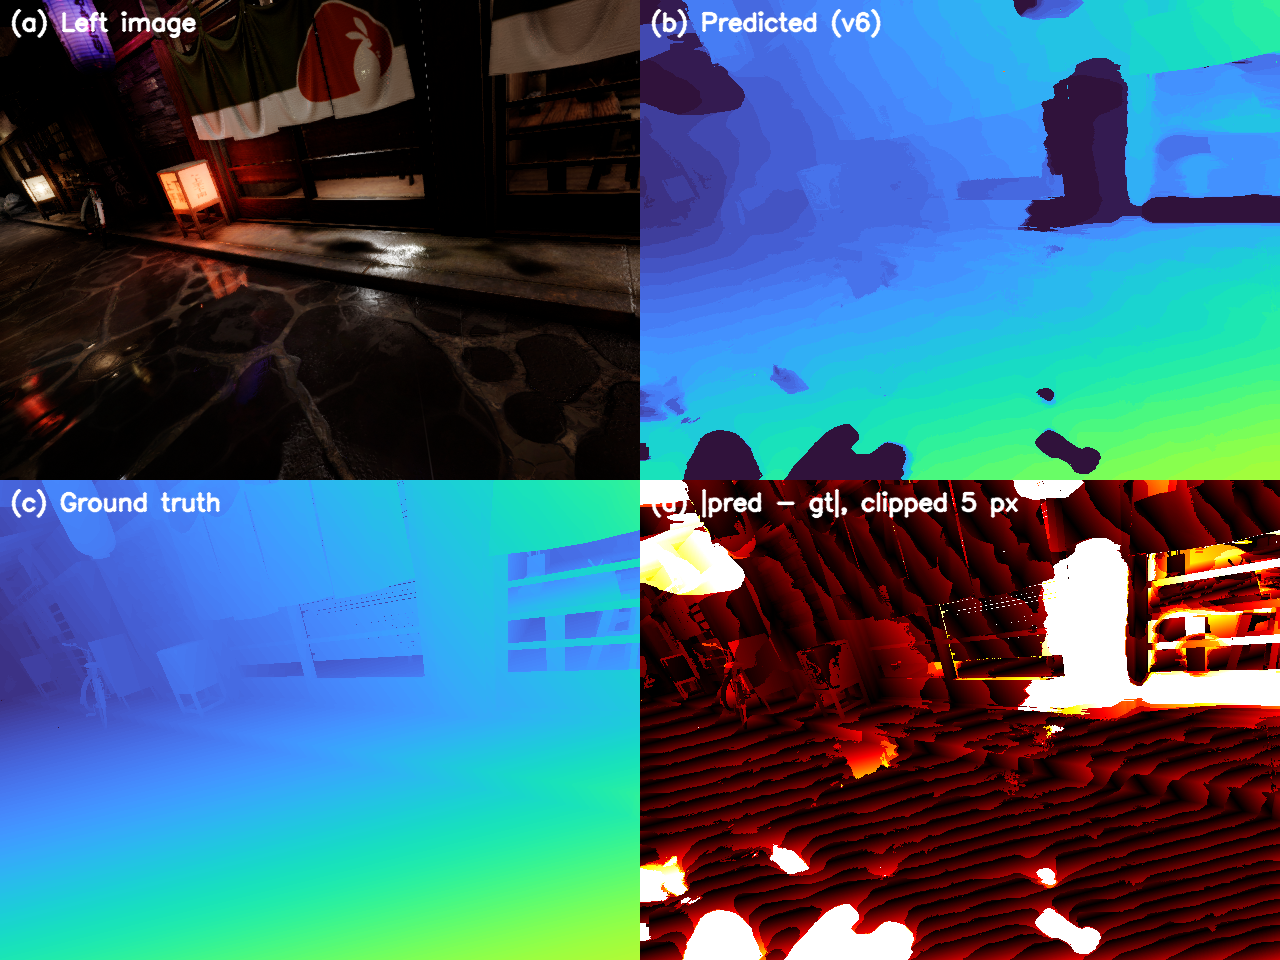
\includegraphics[width=\linewidth]{figures/tartanair_disp_sample.png}
  \caption{frame 30 of japanesealley/Hard/P000：(a) 左圖、(b) v6 預測
  disparity、(c) GT disparity、(d) $|\text{pred}-\text{gt}|$（5\,px clip）。
  錯誤集中在巷尾的遠距離、低紋理區域。}
  \label{fig:bonus-disp-vs-gt}
\end{figure}

\subsection{重建結果}
\label{sec:bonus-results}
\figurename~\ref{fig:bonus-walkthrough} 呈現走訪影片在第 40 frame
的靜止截圖：v6 重建與 GT-depth 上限參考，兩者 mesh 的整體幾何（牆面、地面、
近距離物件）對得起來。完整 mp4 在 \texttt{out/tartanair\_p000\_v6\_100.mp4}
與 \texttt{out/tartanair\_p000\_gt\_100.mp4}。

\begin{figure}[H]\centering
\begin{minipage}[t]{0.48\textwidth}\centering
  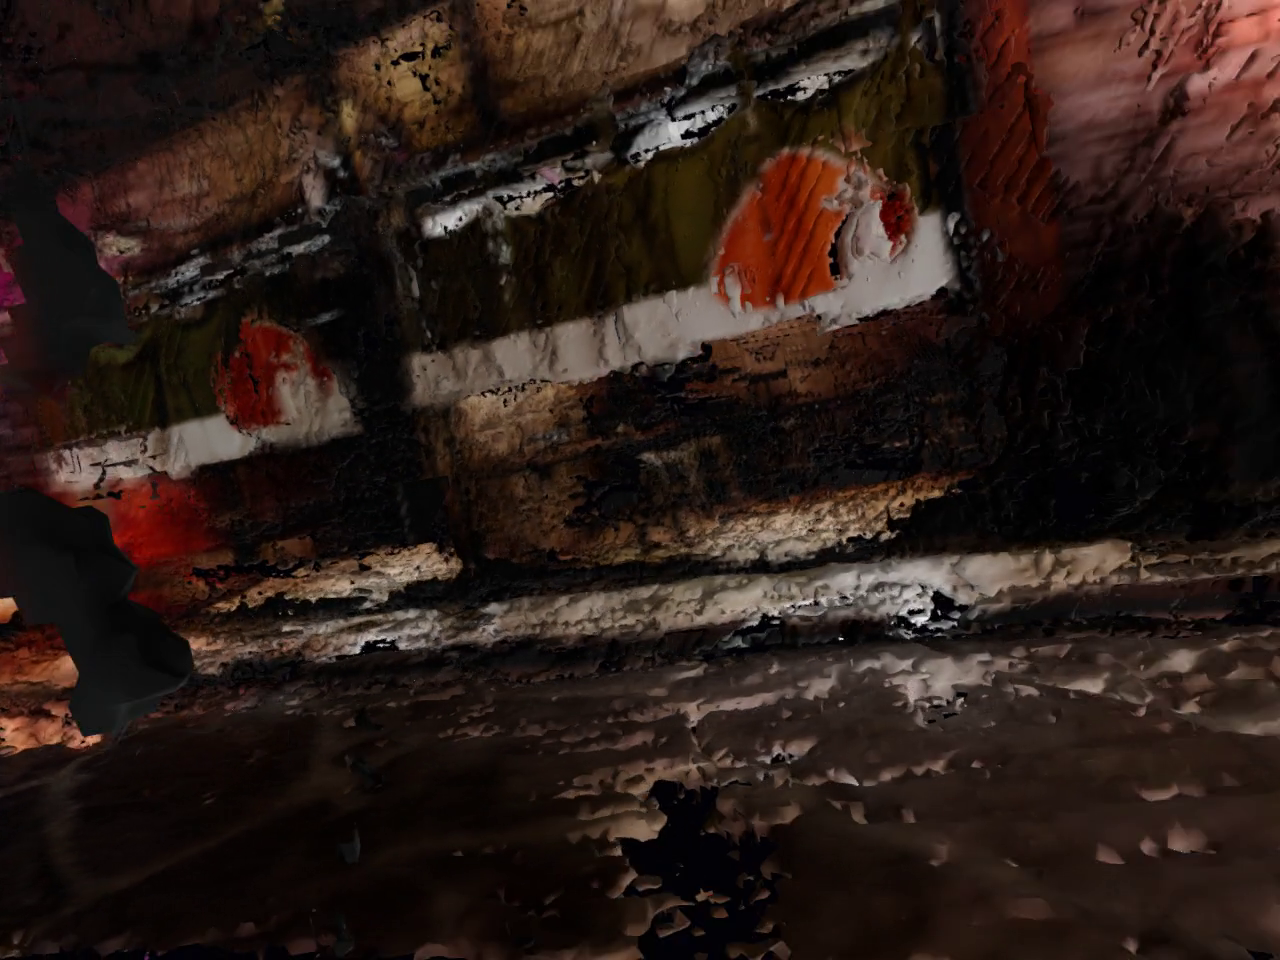
\includegraphics[width=\linewidth]{figures/walkthrough_v6.png}\\
  \small (a) v6 重建（加分題交付物）
\end{minipage}\hfill
\begin{minipage}[t]{0.48\textwidth}\centering
  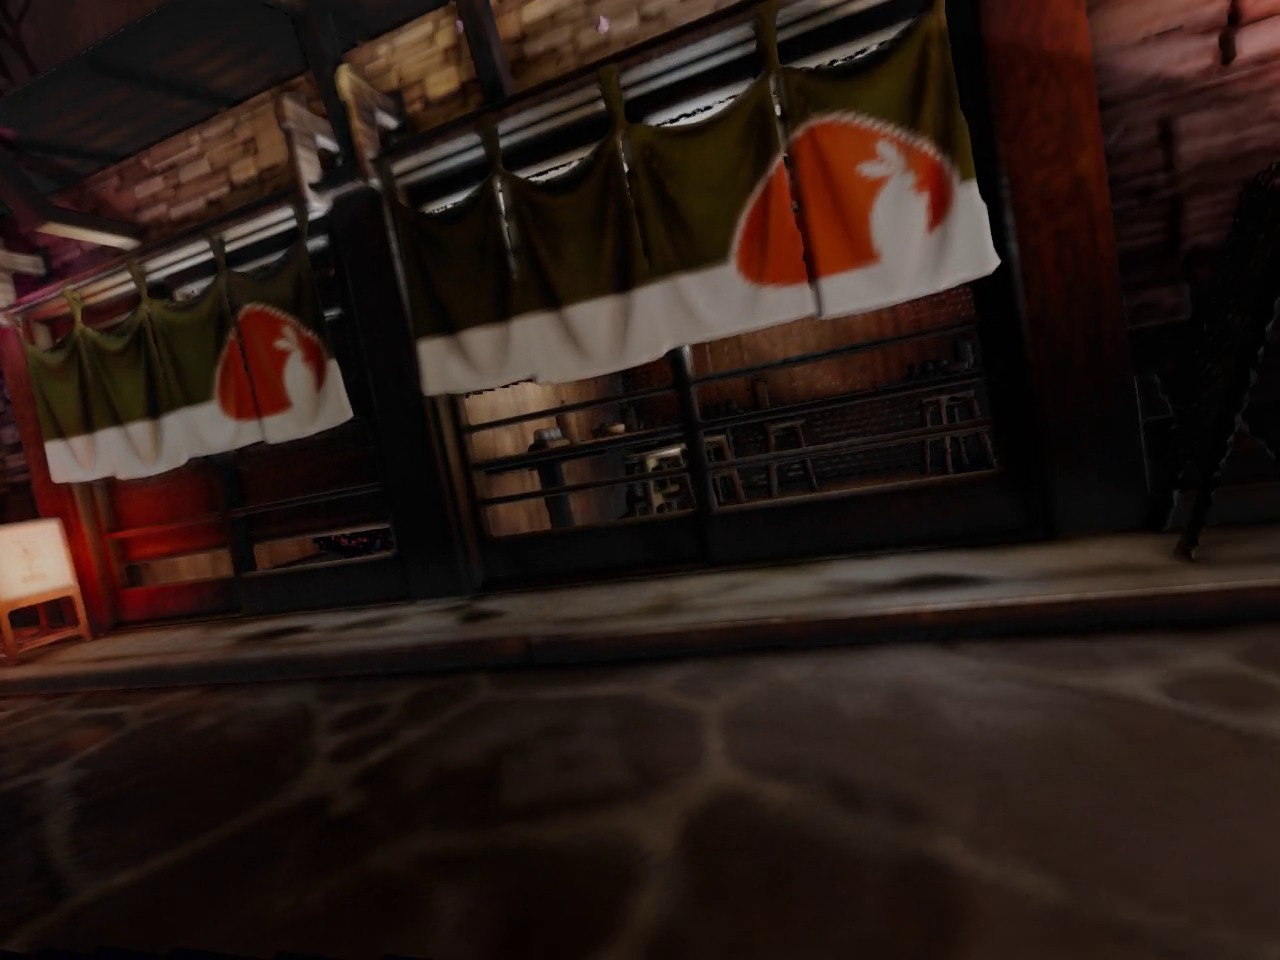
\includegraphics[width=\linewidth]{figures/walkthrough_gt.png}\\
  \small (b) GT depth 上限參考
\end{minipage}
\caption{First-person walkthrough frame 40 截圖。雖然 v6 BPR 仍有 $\sim$20\,\%，
經過 TSDF 多視角融合後表面在視覺上仍清晰可辨——這正是 multi-view fusion
的價值：每幀的隨機 noise 在累積平均下被有效削減。}
\label{fig:bonus-walkthrough}
\end{figure}

\subsection{與 v8 替代版本之比較}
\label{sec:bonus-v8}
我們也試了同學提供的替代實作 \texttt{computeDisp\_v8.py}，其與 v6 的主要差別是：
(i) 多了 parabolic sub-pixel refinement、(ii) WMF 對 sub-pixel disparity 做。
理論上這兩項在 disparity 精度上應該優於 v6 的純整數版本。
但在 TartanAir 上的 BPR 結果：v8 在 1\,px 為 20.26\,\%、3\,px 為 10.75\,\%，
與 v6 \textbf{基本打平}（差距在 $\pm0.05\,$pp 內）。原因清楚：\texttt{computeDisp}
的 API 回傳 \texttt{uint8}，sub-pixel 的小數部分在這個 API 邊界被 clip 掉。
此觀察對下游使用者重要：要享受 sub-pixel 改善，
\textbf{下游必須消費 float disparity}（例如直接拿 cost volume 做 fusion，
或將 disparity 改回 \texttt{float32} 接口）。

\subsection{與業界 SOTA Deep Stereo 之比較}
\label{sec:bonus-sota}

\paragraph{動機。} 古典 stereo 在 TartanAir 上 20\,\% 的 BPR 是\textbf{演算法本身的上限}
還是\textbf{我們實作的短板}？要回答這個問題，最直接的方式是把同一 pipeline 接上業界
SOTA 的深度立體匹配器並對照數字。本節呈現這個對照實驗。

\paragraph{近年 SOTA 景觀（不深入原理）。} 2021 年以降的深度立體匹配演化
可粗分為三條路線：
\begin{itemize}
\item \textbf{Iterative GRU 系列}：RAFT-Stereo~\cite{Lipson2021} 以 ConvGRU 反覆精煉
correlation pyramid 上的 disparity，是後續 iterative 方法的共同基礎。
Selective-Stereo~\cite{Wang2024Selective} 在 GRU 中加入頻率自適應的 Selective
Recurrent Unit (SRU)，2024 年起在 KITTI / Middlebury / ETH3D 多項公開
leaderboard 取得已發表方法第一。
\item \textbf{Geometry Encoding Volume 系列}：IGEV-Stereo~\cite{Xu2023} 把 cost-volume
aggregation network (PSMNet 風格) 與 RAFT 的 iterative refinement 合體；後續
IGEV++~\cite{Xu2025} 進一步引入 multi-range geometry encoding 以處理大 disparity 範圍。
\item \textbf{Foundation Model 系列}：FoundationStereo~\cite{Wen2025} 是 NVIDIA
在 CVPR 2025 的 \textbf{Best Paper Nomination}，主打 zero-shot generalization——以
ViT backbone（搭配 DINOv2~\cite{Oquab2023} 的 monocular prior）加上 1\,M 對
合成立體影像預訓練，在 Middlebury 等 benchmark 上達到 zero-shot 1.1\,\% BP-2
（vs. 先前 zero-shot 最好的 7.5\,\%）。
\end{itemize}

\paragraph{選型理由。} 我們的核心需求是\textbf{在 TartanAir 上做 zero-shot 量化評估}
（在 TartanAir 上 fine-tune 會喪失 BPR 數字的客觀性，等同直接擬合 test set）。
盤點公開 checkpoint 後發現：RAFT-Stereo、IGEV、Selective-Stereo 三家僅釋出
SceneFlow / KITTI / Middlebury 域內權重；唯有 FoundationStereo 因設計初衷
就是 foundation model，公開了在 1\,M 合成資料訓練的 zero-shot checkpoint。
最終選擇 \textbf{FoundationStereo ViT-small}（\texttt{11-33-40/model\_best\_bp2.pth}，
本機 RTX 4090 + 24\,GB VRAM 上推論 \SI{0.28}{\second/frame}）。

\paragraph{整合方式。} 在 \texttt{bonus/deep\_matcher.py} 包成
\texttt{compute\_disparity\_deep(Il, Ir, ckpt)} $\to$ \texttt{np.float32 (H, W)} 簽名的
wrapper；\texttt{bonus/run\_bonus\_tartanair.py} 新增 \texttt{--matcher foundation\_stereo}
flag 走 deep 分支。\textbf{depth conversion、TSDF、render 三層完全沿用 v6 的程式碼路徑
沒有任何改動}——三組 BPR 數字（v6 / v8 / FoundationStereo）落差完全來自 matcher
本身、與下游無關。

\paragraph{結果。} 在 §\ref{sec:bonus-bpr} 完全相同的 100 frame、
\texttt{max\_disp$=64$} 設定下：

\begin{table}[H]\centering
\caption{\texttt{japanesealley/Hard/P000} 前 100 frame，相同 valid mask
（排除 sky 與 $d_{\mathrm{gt}}>\max\!d$ 的像素）。FoundationStereo 為 zero-shot
（沒有任何 TartanAir 微調）。}
\label{tab:bonus-sota}
\begin{tabular}{lcccc}
  \toprule
  Matcher & BPR @ 1\,px (mean) & BPR @ 3\,px (mean) & median @ 3\,px & time / frame \\
  \midrule
  v6 (classical, 我們的 basic 交付物)    & 20.21\,\% & 10.75\,\% & 10.18\,\% & \SI{0.36}{\second} (CPU) \\
  v8 (classical + sub-pixel)             & 20.26\,\% & 10.75\,\% & 10.20\,\% & \SI{0.34}{\second} (CPU) \\
  \textbf{FoundationStereo ViT-small}    & \textbf{3.65\,\%} & \textbf{1.23\,\%} & \textbf{0.91\,\%} & \SI{0.28}{\second} (RTX 4090) \\
  \bottomrule
\end{tabular}
\end{table}

FoundationStereo 把 1\,px BPR 從 20\,\% 砍到 3.65\,\%（\textbf{5.5$\times$ 改善}），
3\,px median 已破 1\,\%。

\begin{figure}[H]\centering
\begin{minipage}[t]{0.48\textwidth}\centering
  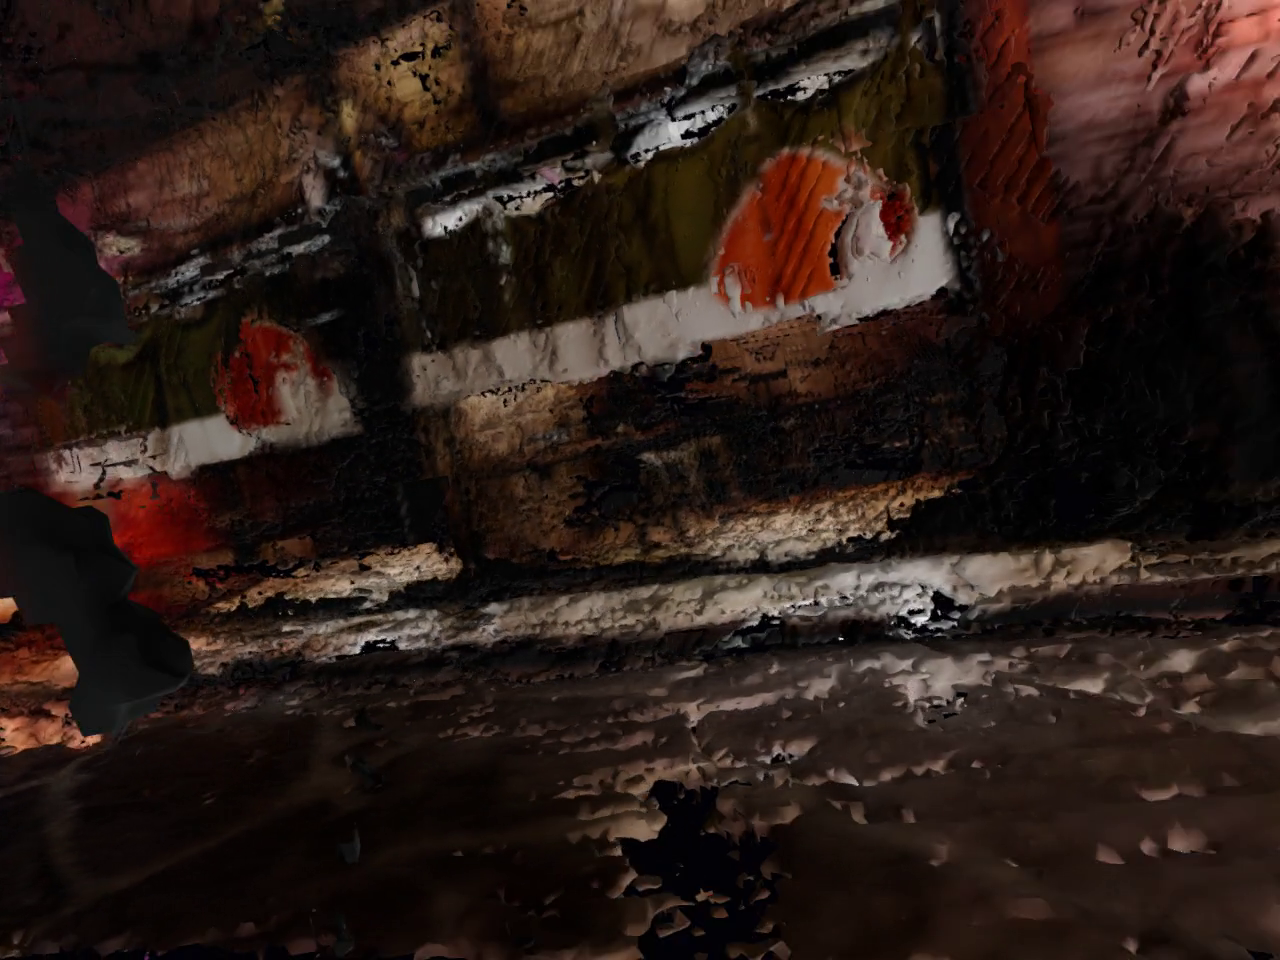
\includegraphics[width=\linewidth]{figures/walkthrough_v6.png}\\
  \small (a) v6 古典 baseline 重建
\end{minipage}\hfill
\begin{minipage}[t]{0.48\textwidth}\centering
  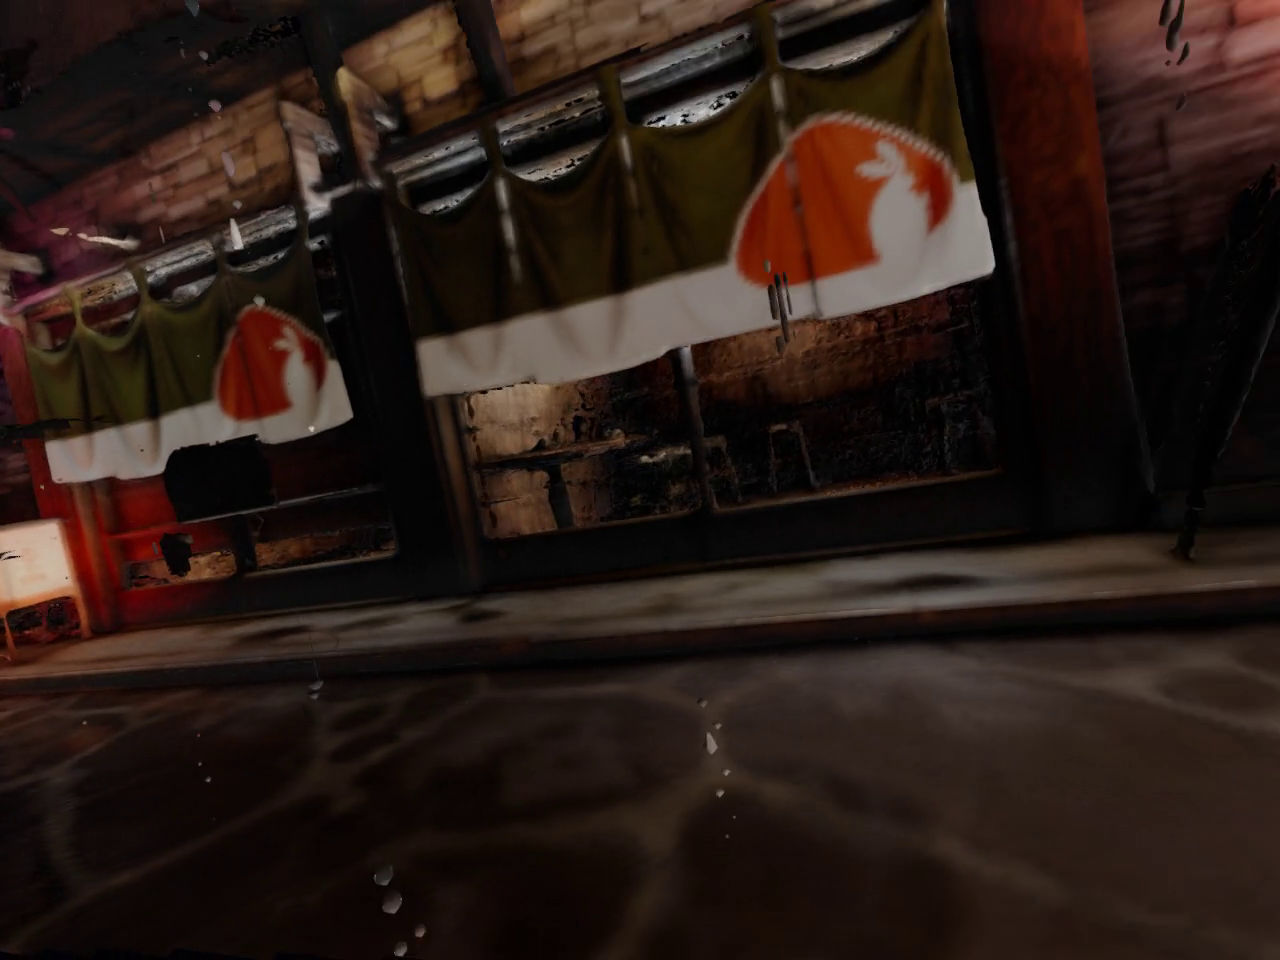
\includegraphics[width=\linewidth]{figures/walkthrough_fs.png}\\
  \small (b) FoundationStereo 重建（zero-shot）
\end{minipage}
\caption{frame 40 first-person walkthrough 對照。FoundationStereo 版本的牆面
更銳利、地面飄浮 outlier 顯著減少；mp4 H.264 壓縮後的大小也從 v6 的
\SI{5.1}{\mebi\byte} 降到 FoundationStereo 的 \SI{2.7}{\mebi\byte}（趨近
GT-depth 上限的 \SI{2.3}{\mebi\byte}），側面驗證 mesh 雜訊大幅下降。}
\label{fig:bonus-fs-walkthrough}
\end{figure}

\paragraph{結論：classical 上限與 deep prior 的角色。} 三個觀察：
\begin{enumerate}
\item \textbf{v6 的 20\,\% BPR 屬演算法上限，非實作短板}：v8 加 sub-pixel 沒有
顯著差別、FoundationStereo 直接掉到 3.65\,\%，這是分布外（synthetic outdoor）
紋理上古典 hand-crafted feature 無法處理的結構性瓶頸。
\item \textbf{Multi-view fusion 是 v6 仍可交付的關鍵}：即便 single-frame BPR 20\,\%，
TSDF 平均掉非系統性 noise 後 mesh 在視覺上仍可辨識（見 §\ref{sec:bonus-results}）；
這也對應到我們把 demonstration video 而非 BPR 數字當作 bonus 的核心交付。
\item \textbf{深度先驗才是突破口}：FoundationStereo 的優勢來自 DINOv2 backbone
+ 1\,M 對合成資料訓練學到的 monocular prior，這在低紋理區域提供了 hand-crafted
Census 沒有的訊號。對未來 work 的啟示是：要進一步提升 bonus pipeline 的重建品質，
方向是接更強的 matcher 與調整下游 fusion（confidence-weighted TSDF）以充分利用
deep matcher 的 sub-pixel 訊號，而非繼續打磨 classical 流程。
\end{enumerate}

% TODO: 開啟下列 bibliography 時，需在 Ref.bib 補上以下新引用：
%   Curless1996, Newcombe2011, Lipson2021, Xu2023, Xu2025,
%   Wang2024Selective, Wen2025, Oquab2023
%   完整 BibTeX 在 report/references.bib 可以直接拷貝。
%\bibliographystyle{IEEEtran}
%\bibliography{./Ref.bib}


\end{document}